\chapter{Computer networks and protocols}
\label{network}

\section{Switched networks}

Packet switched networks, and computer networks in general, have
become an intrinsic part of the computer industry.  With the fall in
their cost and the increase in user-friendly software it is now
possible for people to connect several computers together to form a
network with ease.

Computer networks come in all shapes and sizes and there are a
multitude of methods for connecting two or more computers together.
Each individual network is different, depending on its topology, the
transmission technology and the software running on it.  To fully
understand a network it is necessary to know about each element.

\subsection{Packet switching versus circuit switching}

\subsubsection{Circuit switching}

Circuit switched networks are one of two types of communication
networks, the other being packet switched networks.  Circuit switched
networks are the older of the two as they are the basis of the
telephone system.

Originally telephone networks were based around a central office
where wires from each telephone terminated.  When a call was placed
the operator would physically connect the two wires together.  This
would form an electrical {\em circuit} which would remain intact
throughout the duration of the call.  When the call ended the operator
would disconnect the two wires.  It is not clear where the term
switching came from but it has applied to the operation of connecting
two parties together at a central office from the earliest times of
telephony.

Today the technology is very different but the concepts of circuit
switching remain the same, that is a fixed path between the end
parties is set up at the start of a connection, remains intact
throughout the duration of the call, and is torn down only after the
call has ended.

One important concept with circuit switched systems is that of having
a fixed resource.  Whether you talk or not when using the telephone
does not change the amount of resource being used.  Exactly one
circuit is being used regardless of how much information there is at
any given time, that is the resource usage does not shrink or expand
once the circuit has been set up.

\subsubsection{Packet switching}

Packet switching differs from circuit switching in that whereas a
circuit switching system treats a connection as a continuous stream,
packet switching breaks everything up into discrete, limited size
blocks.  Each block is known as a {\em packet}.  A common analogy is
the idea of a postcard in a postal network.  To send a long message
several postcards have to be written and sent.  Each postcard is
treated independently and they may not arrive in the same order as
they are sent or follow the same route in getting to their
destination.

\subsubsection{Hybrid systems}

A common hybrid system between circuit switched and packet switched
networks is based around the concept of a {\em virtual circuit}.  A
virtual circuit behaves like a standard circuit in that for a
connection between two parties a circuit is formed, remains fixed
throughout the duration of the connection, and is torn down once the
connection has ended.

Virtual circuits differ in that rather than having a fixed resource
throughout the duration of the connection to support a continuous
stream of data the input is broken up into packets.  Each packet
follows a set route decided upon at the creation of the circuit, but
if there is no input to be transmitted then no packets are sent.  This
way resources only need to be used when something is to be
transmitted, the resources growing or shrinking as needed.

The idea is to keep the simplicity of a fixed circuit while trying to
maximise the utilisation of limited resources.  While it looks like a
circuit it suffers from the major problem of a packet switched system,
that is congestion.  With proper circuit switching if inadequate
resources are available, a connection will fail when the system
attempts to open it (as in a busy signal or trunk full signal
experienced with the telephone system) but in packet switching
resources are only used when a packet is sent so having inadequate
resources is only discovered when a packet is actually sent.  A
supplier may allocate more virtual circuits then the number of actual
physical ones, assuming that not every connected party will want to
send something at any given point in time.  If too many parties do try
to send something at the same time then the network's resources will
be exceeded causing some packets to be dropped (the packet is ignored
by the system and ceases to exist) or delayed.

Virtual circuit based networks are called {\em connection oriented
packet switched networks}.  In contrast packet switched networks where
each packet is completely self contained are called {\em
connectionless packet switched networks} or just {\em connectionless
networks}.

\subsubsection{Datagram networks}

Connectionless packet switched networks are often called {\em
datagram} networks.  Because the packets are self contained they are
often thought of as a individual blocks of data travelling through
the network and are hence called datagrams.  Most datagram networks
follow the {\em hop-by-hop} paradigm, that is each intermediate system
redirects datagrams without respect to the datagram's previous travels
or its further travels.  This implies datagrams do not keep a history
of their travels but rely on the co-operation and co-ordination of
intermediate systems to relay them to their destination.

\section{Network protocols}

A {\em protocol} is a set of rules on how to behave in given a set of
circumstances.  Protocols generally come grouped together as a {\em
protocol family} and are normally arranged in a semi hierarchical
fashion, with many protocols relying on others to do work for them
while being relied on by other protocols.  This pseudo hierarchy for a
given protocol family is called a {\em protocol stack}.

\begin{figure}
\begin{center}
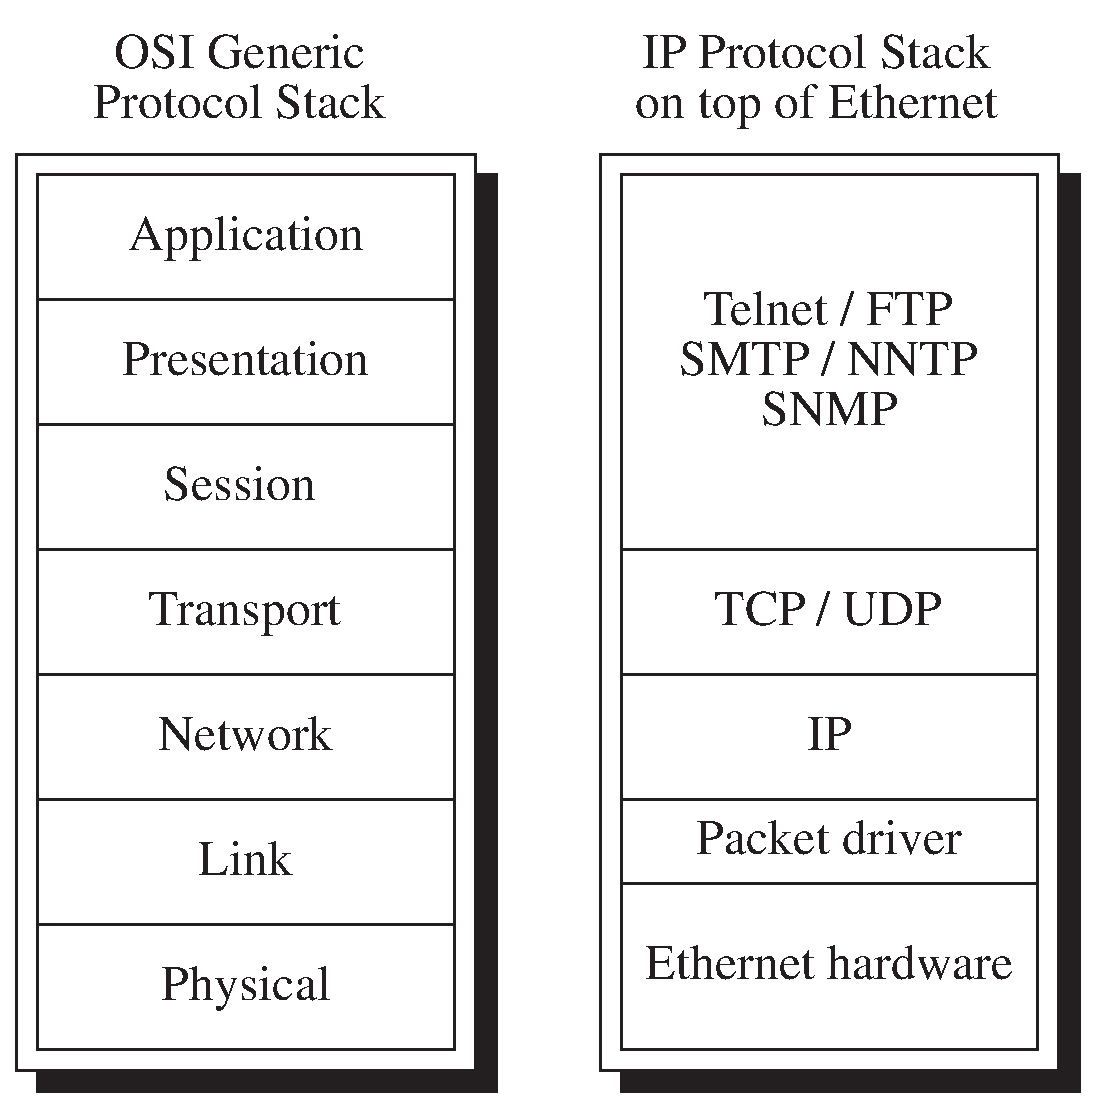
\includegraphics[height=3in]{pics/pstack.eps}
\end{center}
\caption{OSI and TCP/IP Protocols Stacks}
\label{network:pstack}
\end{figure}

Throughout the history of computing there have been many network
protocols, most of them proprietary to specific systems.  As market
forces drive networks towards greater connectivity many of these
protocols have fallen by the wayside, leaving a handful of system
specific protocols and two major `open' systems.  Common network
protocols include SNA (Systems Network Architecture) from IBM, DECnet
from Digital Equipment Corporation, IPX (Netware) from Novell and
AppleTalk from Apple Computer.  The two major open systems protocols
are TCP/IP (Transmission Control Protocol / Internet Protocol) and OSI
(Open System Interconnection) (See Figure~\ref{network:pstack}).

\subsection{Internet Protocol}
\label{network:ip}

\subsubsection{History and comments}

The Internet Protocol, commonly known as IP, developed from ARPANET
(Advanced Research Project Agency NETwork), one of the earliest packet
switching networks developed \cite{RFC:791}.  ARPANET was funded by
the United States Department of Defence, who required a computer
network able to survive a limited nuclear attack.  For this reason
emphasis was placed on distributing decision making (as any
centralised system would be an obvious target) and reliability in
extreme circumstances.

ARPANET no longer exists but has been replaced by the {\em Internet},
a world wide network of networks, all using IP as their base
technology.  IP is a datagram protocol and is usable over a very wide
range of transmission technologies.

\subsubsection{Deployment within the University}

IP addresses are 32 bits wide and are split up into two parts, the
first being the network address and the other the host address.  IP
routes packets to the network level where it expects to be able to
communicate directly to the host.  Originally IP addresses were split
up into classes, for example class B addresses had 16 bits for the
network address and 16 bits for the host address, with class C having
24 bits for the network address and 8 bits for the host address.

The class of the address was encoded into the high bits of the address
so a router could tell how many bits it needed to make a routeing
decision on.  This fixing of the address part sizes was extremely
limiting so it was replaced by a 32 bit contiguous mask.  The mask
indicates which part of the address is the network part.

TCP/IP is deployed throughout the university and is available to all
departments.  Currently the university has a class B address which is
split up into 256 class C addresses using address masks.  This is
important for routeing packets within the university network.  From the
outside the university has a single 16 bit network address {\tt
130.216.0.0} (the full address is always used even though the only the
top 16 bits are significant, non significant bits are set to zero) but
inside the university all networks addresses are 24 bits wide, for
example mathematics is {\tt 130.216.15.0}.

\subsection{AppleTalk}
\label{network:appletalk}

\subsubsection{History and comments}

{\em AppleTalk} is the network protocol suite developed by Apple
Computer Inc. when it released the Macintosh \cite{AppleTalk:Apple}.
It was developed specifically for small local area networks.
Originally it only ran over {\em LocalTalk}, a bus topology physical
network.  LocalTalk has a very low bandwidth by today's standards but
it didn't require any extra hardware since all Macintoshes come with
it built in.  In later versions {\em EtherTalk} was added.  This
enabled the AppleTalk protocols to run over standard Ethernet.

It is mainly used for connecting Macintoshes to file servers and
printers.  Over small networks (up to the size of a campus network)
the protocol runs without difficulty.  It has a distributed directory
service which makes using it simple, but limitations in that protocol
now limit how large the network can grow.

AppleTalk cannot easily be used over wide area networks.  This is
mainly to do with limitations in its ability to address physical
entities on the network.  Also, the directory service breaks down over
slower links.

AppleTalk splits the network up into logical {\em zones}, where one or
more physical segment belongs to a zone.  Zones are not used in packet
routeing but are for human use only, dividing the network up logically
to simplify directory lookups, that is AppleTalk has a two level
directory consisting of zones and logical entities, which belong to
exactly one zone.  Because zones cannot belong to other zones,
connecting two separate AppleTalk networks, say two universities, is
infeasible without extreme care.

\subsubsection{Deployment within the University}

AppleTalk is also widely deployed throughout the campus.  The majority
of the network is over Ethernet with some outlying sections using
LocalTalk.

\subsection{IPX}
\label{network:ipx}

\subsubsection{History}

IPX, or {\em Internet Packet eXchange} is the network layer protocol
used by {\em Netware} \cite{Novell:IPX}.  Netware is a product from
Novell Inc which provides file server and remote printing services.  A
Netware network is a collection of file and printer servers connected
together using IPX.  Client machines, running MS-DOS or Windows,
connect to a server, and software on the client machine makes the
remote file systems behave as if they were connected locally.

IPX itself is a very simple protocol with a two level addressing
system.  Physical segments are each assigned an address, and machines
on the physical segments are addressed using their hardware address.
This simplicity reduces the amount of computing required to send each
packet, but limits the flexibility of the protocol.  IPX runs almost
exclusively over Ethernet.

\subsubsection{Deployment within the University}

IPX can go over any Ethernet segment provided it is able to be routed
onto it.  Most departments have enabled IPX routeing and often their
Novell servers also do IP and AppleTalk routeing.

Netware also places a non trivial load on the network because every
two minutes (or however long the administrator sets it) the router
broadcasts information about every Netware service available.  When
the number of file servers exceeds twenty this information becomes
large in size.  Currently the information is about 500 kilobytes in
size.  On busy networks such as student labs, this is unwelcome extra
traffic.

\section{Physical transmission media}

While the number of common network protocols is less than ten the
number of ways of transmitting digital information is at least five
times this.  Each method differs in behaviour and hence alters the
characteristics of traffic using it.  Fortunately most methods fall
into broadly defined groups, with each member of the group exhibiting
similar behaviour.

\subsection{Analog and digital transmission technologies}

All data transmitted is electro-magnetic energy at some stage (whether
it be light, radio or signals along copper wire) and as such is analog
in nature.  All modern data communication is digital in nature so
transmission requires signals to be encoded.  The term {\em bandwidth}
originally came from broadcasting, where it determined how large a
slice of the radio spectrum a transmitter could use.  This in turn
governed the frequency range of the transmission and how much
information could be sent in a given period of time.  The modern usage
still measures the rate at which data can be sent but unless specified
should not be seen as relating to the underlying analog technology.

\subsection{Point to point connections}

Point to point connections are the easiest to visualise.  {\em
Transceivers} (devices which both transmit and receive data) are
placed at either end of a cable.  If both transceivers can send
simultaneously then the medium is said to support {\em full duplex}
transmission otherwise the medium is said to be {\em half duplex}.

Point to point connections have two major characteristics.  The first is
bandwidth, measured in bits per second (bps) and in magnitudes of
multiples of one thousand (this is different from computers where
orders increase in multiples of $2^{10}$).  The other is {\em
latency}, which is a measure of delay between when data is sent and
subsequently received.  This is normally measured in the orders of
seconds (for example, milliseconds or microseconds).

\subsubsection{Framing}

Data is not sent in a raw stream but is encapsulated into discrete,
limited size packets, known as {\em frames}.  Framing the data avoids
excessive error propagation as well as providing information for
clock synchronisation.  Frames may also contain information about
addressing data to a particular transceiver and error correction.

Frame sizes vary from as little as 53 {\em octets} (an octet is eight
bits,  the term byte is normally used with respect to computers) to
over 8192 octets (8 Kbytes).  It is important for protocols using a
particular transmission medium to match their packet sizes to that of
the transmission frames.

\subsubsection{Serial and parallel connections}

Modern computers normally store data in blocks of 32 or 64 bits.  When
transmitting these blocks inside the computer they are sent in {\em
parallel}, that is to say 32 or 64 separate connections are used, with
each bit being sent simultaneously.  This means that large amounts of
information can be sent rapidly.

When sending data between two computers physical wires are required
making very wide parallel cables extremely expensive.  While eight bit
wide parallel cables are common they only ever extend a distance of
metres.  Wider cables are now being used to connect computers to high
speed peripherals but only up to a distance of one or two metres.

Over longer distances these blocks of data are sent bit by bit in
sequence.  This is known as {\em serial} transmission and only
requires two copper wires or one optical fibre per direction.  Over
any significant distance it is cheaper to make serial transmission
faster than to make parallel cables wider.

\subsection{Contention and bandwidth allocation}

When two or more parties attempt to simultaneously use a limited
resource then one or more must miss out.  This fighting is called {\em
contention} and the process for deciding who finally gets the resource
is called {\em contention resolution}.  Contention occurs in many
places in computing and specifically in data transmission where it is
associated with transmitters wanting to simultaneously send data with
limited bandwidth.

Contention can be resolved in a number of ways, each having advantages
and disadvantages.

\begin{itemize}

\item Stations are given set priorities.  If a station with a higher
priority wants to send then any sender which is lower must stop.  This
is called a {\em priority based} system.

\item A centralised station gives the right to send to subservient or
slave stations.  This is called {\em polling}.

\item The right to send is passed from station to station in an
orderly fashion.  This method is called {\em token passing}.

\item Two or more stations attempt to send and collide.  They then
fight among themselves until there is a winner who gets the right
to send.  These are called {\em contention} networks.

\item Data is transmitted in buckets and stations wanting to send must
let a certain number of empty buckets pass before they can use one.
This broadly falls into the category of {\em distributed queue}
networks.

\end{itemize}

\subsection{Broadcast media}

Radio, television and satellite are all broadcast media.  All
receiving stations get an identical signal from the sender.  This can
in principle be extended to include all receivers connected to a
single piece of wire.

This idea can be taken further and we may define a broadcast network
as a network such that any station can send a single packet to every
other connected station, which will receive an identical copy of that
packet.  This definition includes all physical topologies where
signals are propagated to every connected station.  Hence we can
include such networks as token ring and dual bus networks.

Broadcasting is very useful for sending information to every station
and is very efficient provided the transmission technology is based on
network wide signal propagation, where broadcast essentially comes for
free.  When the physical technology does not allow for broadcasting it
must be simulated.  This means every station wanting to receive
broadcasts must have the message individually sent to them.  For any
network of non trivial size this can become hugely expensive in
bandwidth.

\subsection{Common transmission technologies}

Below is a quick overview of common transmission technologies.  Full
details of some of them will be given in later chapters.

\subsubsection{Ethernet}

\begin{figure}
\leavevmode
\epsffile{pics/enet.eps}
\caption{Ethernet II and IEEE 802.3 Frames}
\label{network:enet}
\end{figure}

Ethernet is a contention based broadcast network designed to work over
short distances (tens to hundreds of metres).  It is the most widely
deployed transmission technology in computer networking with equipment
cheaply and widely available.  Its relative ease of installation and
maintenance has lead to it becoming the baseline technology within the
micro computer industry.  It is now known as IEEE 802.3, which is the
standard which currently defines it \cite{Digital:Ethernet}
\cite{IEEE:Ethernet}.  The raw transmission speed is normally 10 Mbps
but work is proceeding on defining a 100 Mbps standard.

The original Ethernet is now known as Ethernet II or Blue Blue
Ethernet, after the colour of the book which defined the standard.  It
is physically compatible with IEEE 802.3 but has a different frame
structure (See Figure~\ref{network:enet}).  Ethernet II is still
commonly used, especially with respect to TCP/IP.

\subsubsection{Token ring}

Token ring, specifically the standard IEEE 802.5, is a token passing
broadcast network \cite{IEEE:Tokenring}.  It is not as common as
Ethernet and its normally associated with IBM equipment.  Token ring
normally has a raw data rate of either 1, 4 or 16 Mbps.  Note it is
unwise to make a direct comparison between these rates and that of
Ethernet as raw transmission rate is a poor indicator of true
throughput.

\subsubsection{FDDI}

FDDI, or Fibre Distributed Data Interface, is another token passing
network.  It is very similar to IEEE 802.5 except it runs on optical
fibre rather than copper wire.  Raw transmission rate (as seen by a
connected station) is 100 Mbps.

\subsubsection{PPP and SLIP}

While not physical technologies these define how data is to be sent
along serial connections.  SLIP (Serial Line Internet Protocol) is a
De-facto standard used because of its simplicity and wide availability
\cite{RFC:1055}.  PLIP (Parallel Line Internet Protocol) is an
analogous standard for parallel connections but is fairly uncommon.
PPP (Point to Point Protocol) is a full and complete standard for
transmitting packets over point to point connections \cite{RFC:1661}.
It provides Data Link layer functions such as error checking for the
link.

\section{The University campus network}

The campus network is a collection of physical networks connected
together via routers.  A majority of the physical networks are
Ethernet, either using copper wire or point to point Ethernet
connections using optical fibre.

\begin{figure}
\leavevmode
\epsffile{pics/uni-network-map.eps}
\caption{Topological map of the University of Auckland Network}
\label{map:uni}
\end{figure}

\subsection{Computer Centre network}

\begin{figure}
\leavevmode
\epsffile{pics/subnets-1-2-map.eps}
\caption{Topological map of part of the Computer Centre Network}
\label{map:ccnet}
\end{figure}

The computer centre network did have five sub-networks when the
experiments were being performed.  Since then a major re-arrangement
has taken place; this is not reflected here.

The network consisted of subnet 1, which connected the staff offices
and the VAX cluster, subnet 2, which held the computer centre Netware
servers and subnet 3 which has the Unix hosts.  There was also a
subnet 9 which served the terminal room containing PCs with Netware
and Macintoshes.

\subsection{Gateway network}

\begin{figure}
\leavevmode
\epsffile{pics/gateway-net-map.eps}
\caption{Topological map of the University Gateway Network}
\label{map:dmz}
\end{figure}

The gateway network, commonly known as the DMZ (Demilitarized Zone)
network, is used to separate the University network, the Auckland
local networks connected though common carrier dialup and leased
lines, and the frame relay connection to the rest of New Zealand and
the world.
